% !TEX root = Dokumentation_PMP.tex
\section{Projektführung}
Die nachfolgenden Abschnitte dienen der Projektführung und sollen das Projektmanagement unterstützen. Dabei werden der zeitliche Rahmenplan erläutert und die Risiken im Zusammenhang mit dem Projekt beleuchtet.
\subsection{Rahmenplan}
Um einen Überblick über den geplanten Projektverlauf zu bekommen, ist nachfolgend
ein Rahmenplan definiert.
\begin{figure}[H]%Position festigen
\centering
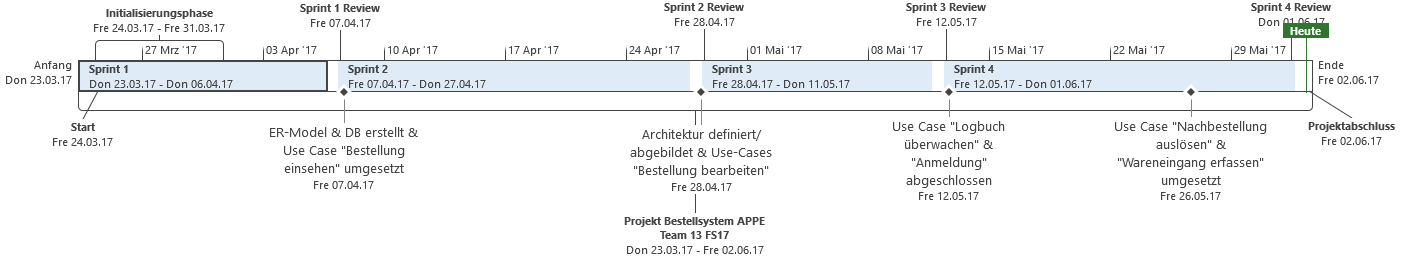
\includegraphics[width=1.0\textwidth]{Images/GroberTerminplan.png}
\label{fig:title}
\end{figure}
Das Projekt wird vom 23.03.2017 bis am 02.06.2017 durchgeführt. Zur regelmässigen Kontrolle \& Planung wird die Projektdauer in vier Entwicklungssprints unterteilt. Auf dem Weg zur finalen Version werden ebenfalls vier Meilensteine wie folgt gesetzt:
\begin{enumerate}
\item Meilenstein 1 \textit{ER-Modell \& DB erstellt \& Use Case 'Bestellung einsehen' umgesetzt}\\
Neben den Initialisierungsaufgaben wie Erstellung PMP \& SysSpec und initiale Anforderungsaufnahme liegt die DB anhand des vorgängig erstellten ER-Modell vor. Weiter ist der erste Use Case 'Bestellungen auflisten' umgesetzt
\item Meilenstein 2 \textit{Architektur definiert \& Use Case 'Bestellung ansehen \& bearbeiten' umgesetzt}\\
Neben der Layer- \& Tierarchitektur, Komponentenschnitt ist der Use Case 'Bestellung bearbeiten' vollständig umgesetzt. 
\item Meilenstein 3 \textit{Use Case 'Nachbestellung' \& 'Anmeldung' umgesetzt} \\
Alle Use Cases bis auf 'Logbuch überwachen' sind umgesetzt. Erste Integrations- \& Systemtests sind ausgeführt.
\item Meilenstein 4 \textit{Use Case 'Logbuch überwachen' \& Dokumentation abgeschlossen}\\
Neben dem letzten Use Case 'Logbuch überwachen' werden alle Integrations- \& Systemtests durchgeführt. Abschliessend liegen die SysSpec und der PMP vor.
\end{enumerate}
\clearpage
\subsection{Projektkontrolle}
In der Projektkontrolle sollen Abweichungen zwischen SOLL- und IST-Zustand aufgedeckt werden. Der Zustand bezieht sich auf den Projektfortschritt. In jedem Sprint werden Arbeitspakete definiert und mit einem bestimmten Aufwand (in Stunden) versehen. Die Arbeitspakete werden jeweils im Rahmen des Sprintreviews auf der Umsetzung kontrolliert und der Status über ScrumDo nachgeführt und mit dem ProductOwner verifiziert.
\subsection{Risikomanagement}
Die Projektrisiken wurden evaluiert und in Tabelle \ref{tab:risklist} dargestellt. Die einzelnen Risiken wurde auf ihre Wahrscheinlichkeit und Auswirkung bewertet und in der folgender Grafik klassifiziert. Zusätzlich wurde je eine Massnahme zur Prävention und zur Verringerung / Eindämmung definiert
\begin{table}[H]
\begin{tabular}{ | p{0.25\textwidth} | p{0.13\textwidth} | p{0.09\textwidth} | p{0.44\textwidth} | }
\hline \rowcolor{gray!50}
%Titelzeile
	\textbf{Risiko} &
	\textbf{Auswirkung}	 	 &
	\textbf{Schaden}	 	 &
	\textbf{Massnahme}
	\\ \hline
%Zeile
	Projektmitglied fällt für mehr als zwei Wochen aus &
	kritisch &
	vorstellbar &
	\begin{tabular}{l}
		- Planbare Absenzen frühzeitig melden\\
		- Regelmässiger Abgleich Arbeitsstand\\
		im Team
	\end{tabular}
	\\ \hline	%Untere Abgrenzung
%Zeile
	EnterpriseLab steht während	einer Woche	oder mehr nicht	zur Verfügung &
	katastrophal &
	vorstellbar &
	\begin{tabular}{l}
		- Lokale Kopie der Artefakte vorhanden\\
		- Lokale Kopien auf GitHub pushen \\
		und verwenden
	\end{tabular}
	\\ \hline	%Untere Abgrenzung
%Zeile
	Eingesetzte Frameworks zu aufwändig &
	geringfügig &
	vorstellbar &
	\begin{tabular}{l}
		- Nicht von Tools \& unnötige Features\\
		 ablenken lassen\\
		- Unnötige Technologien ausschliessen
	\end{tabular}
	\\ \hline	%Untere Abgrenzung
\end{tabular}
\label{tab:risklist}
\caption{Risikoliste}
\end{table}
Im Rahmen der Projektdurchführung ist das Risiko 1 'Projektmitglied fällt aus' eingetroffen. Severin G. war unfallbedingt für zwei Wochen nicht im Projekt einsetzbar. Die anstehenden Aufgaben wurden daher auf die anderen drei Teammitglieder verteilt und nicht prioritäre Arbeiten auf den nächsten Sprint verschoben.